\section{Run-time View}
These sequence diagrams show how the different components interact through each other when the main features are used by various actors.
\subsection{Login}
A Third Party browses the web page login of the TrackMe web application to authenticate itself and could be able to use the provided services. It inserts its credential (username and password). The Request Module checks if the inserted data match with an existent account, and if it is recognized, logged in it.
\begin{figure}[H]
    \centering
    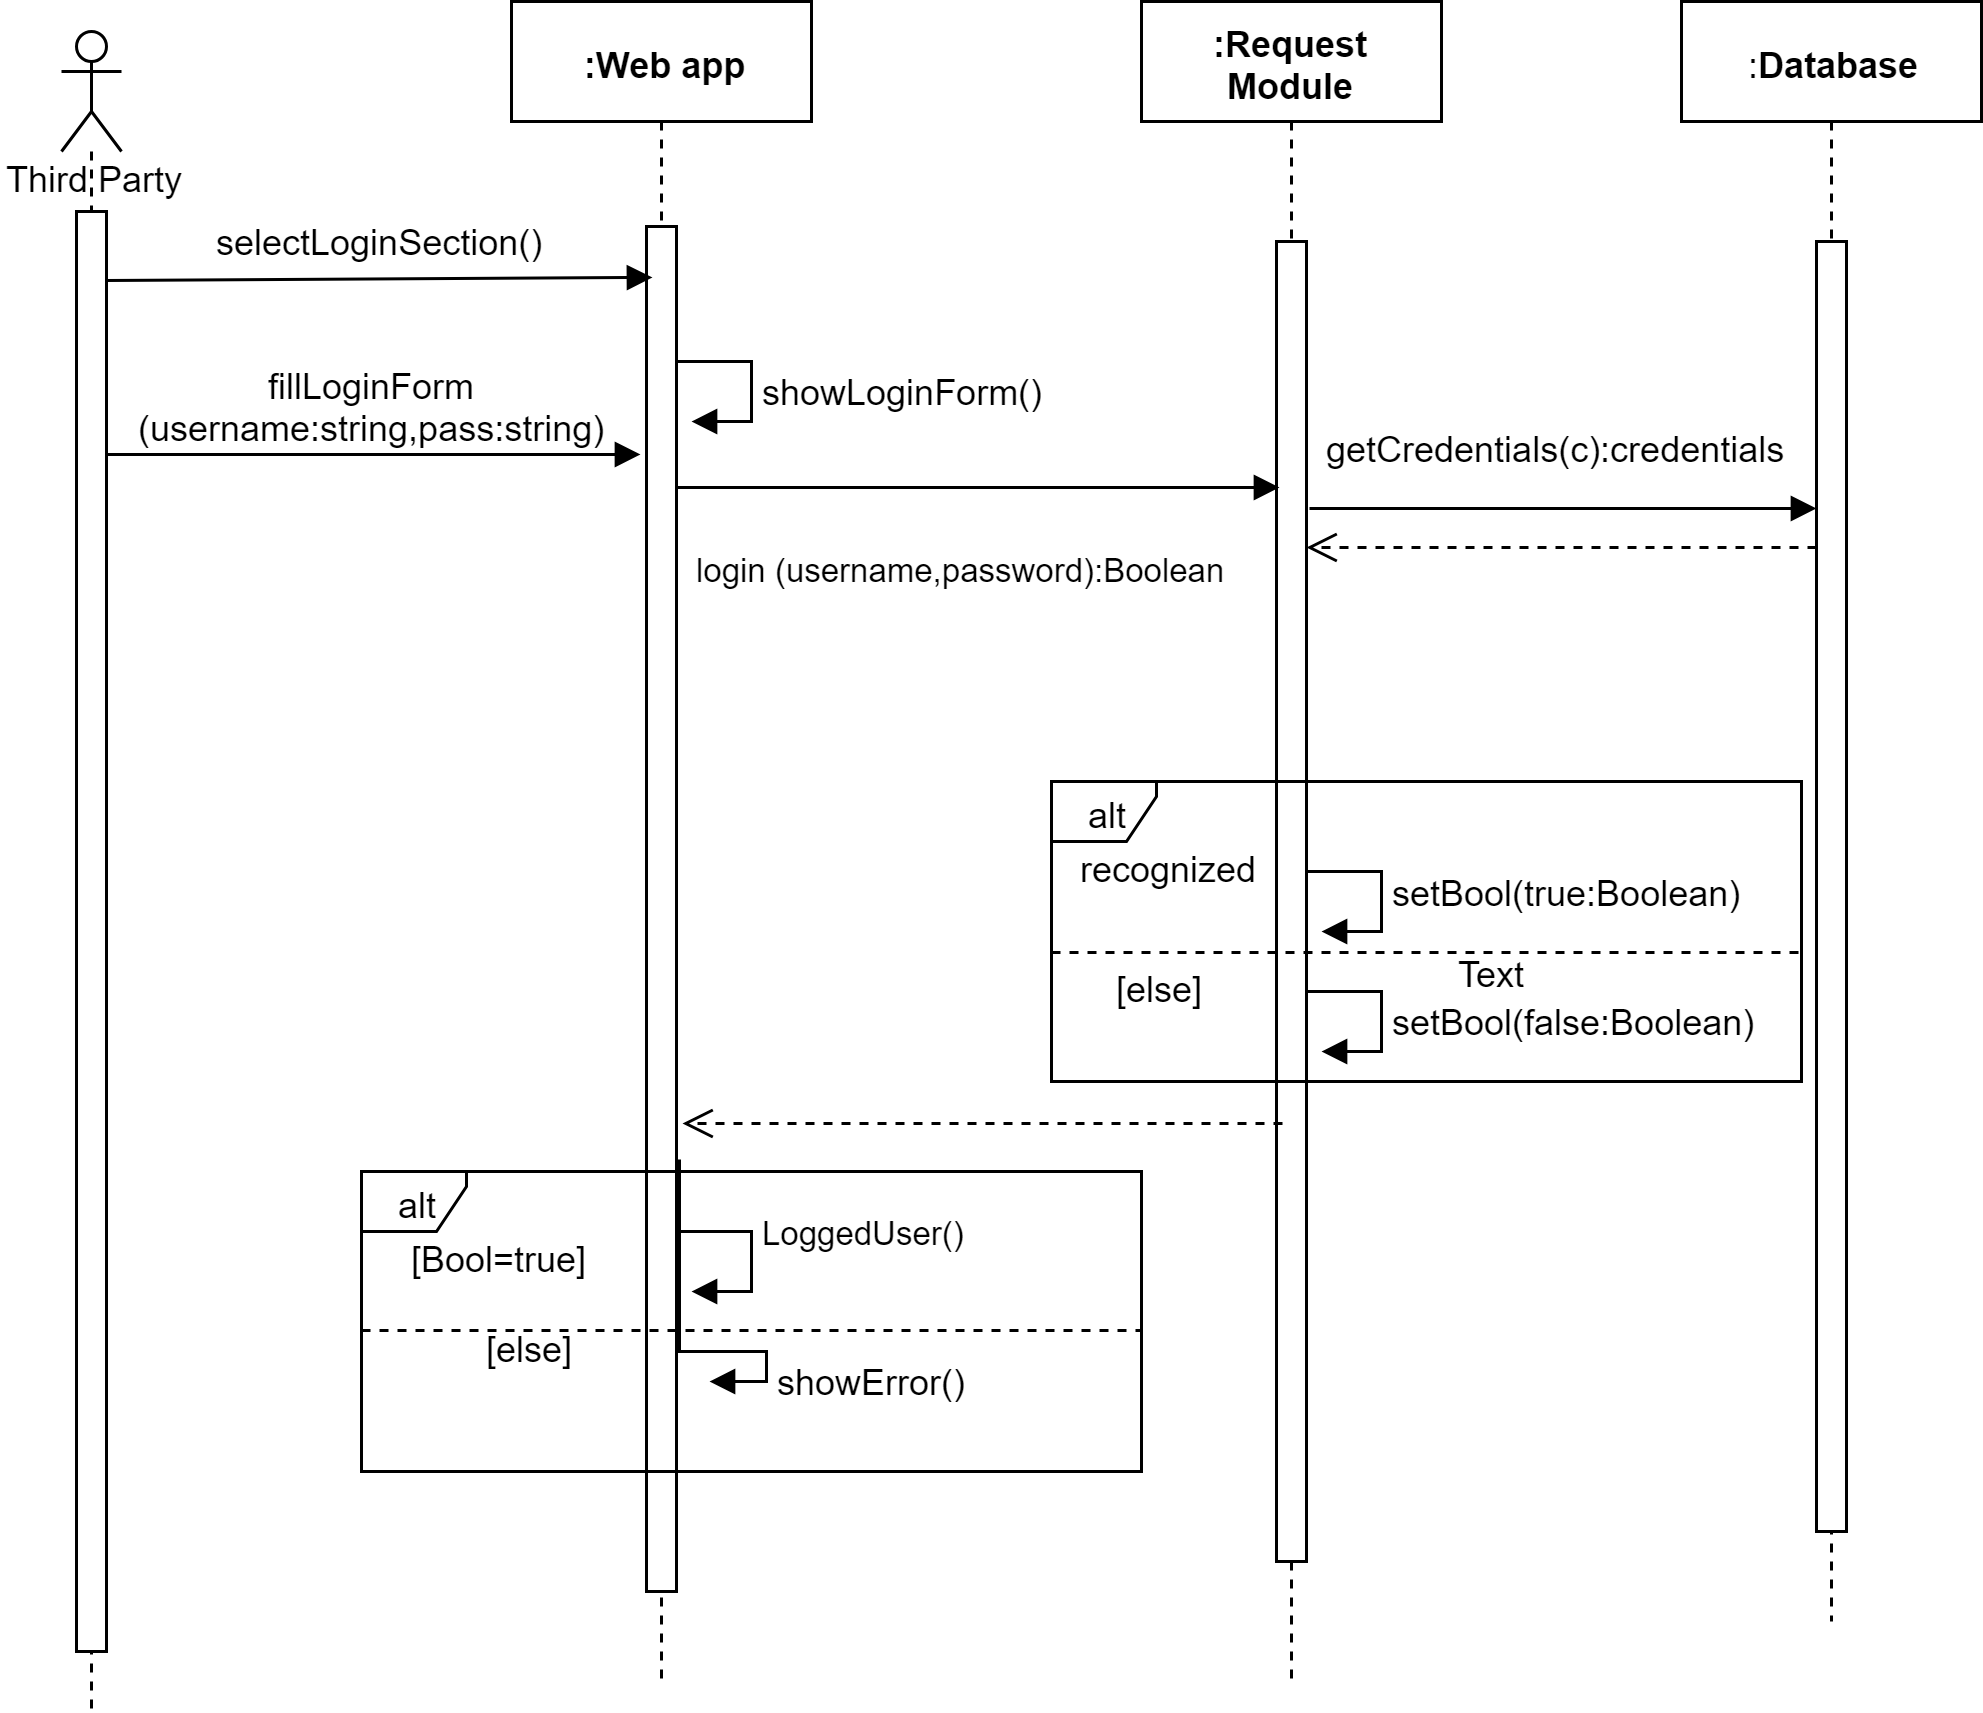
\includegraphics[scale=0.35]{DD/Pictures/login.png}
    \caption{Login sequence diagram}
\end{figure}
The Login process for a User of the mobile application is the same.
\subcaption{User request}
\begin{figure}[H]
    \centering
    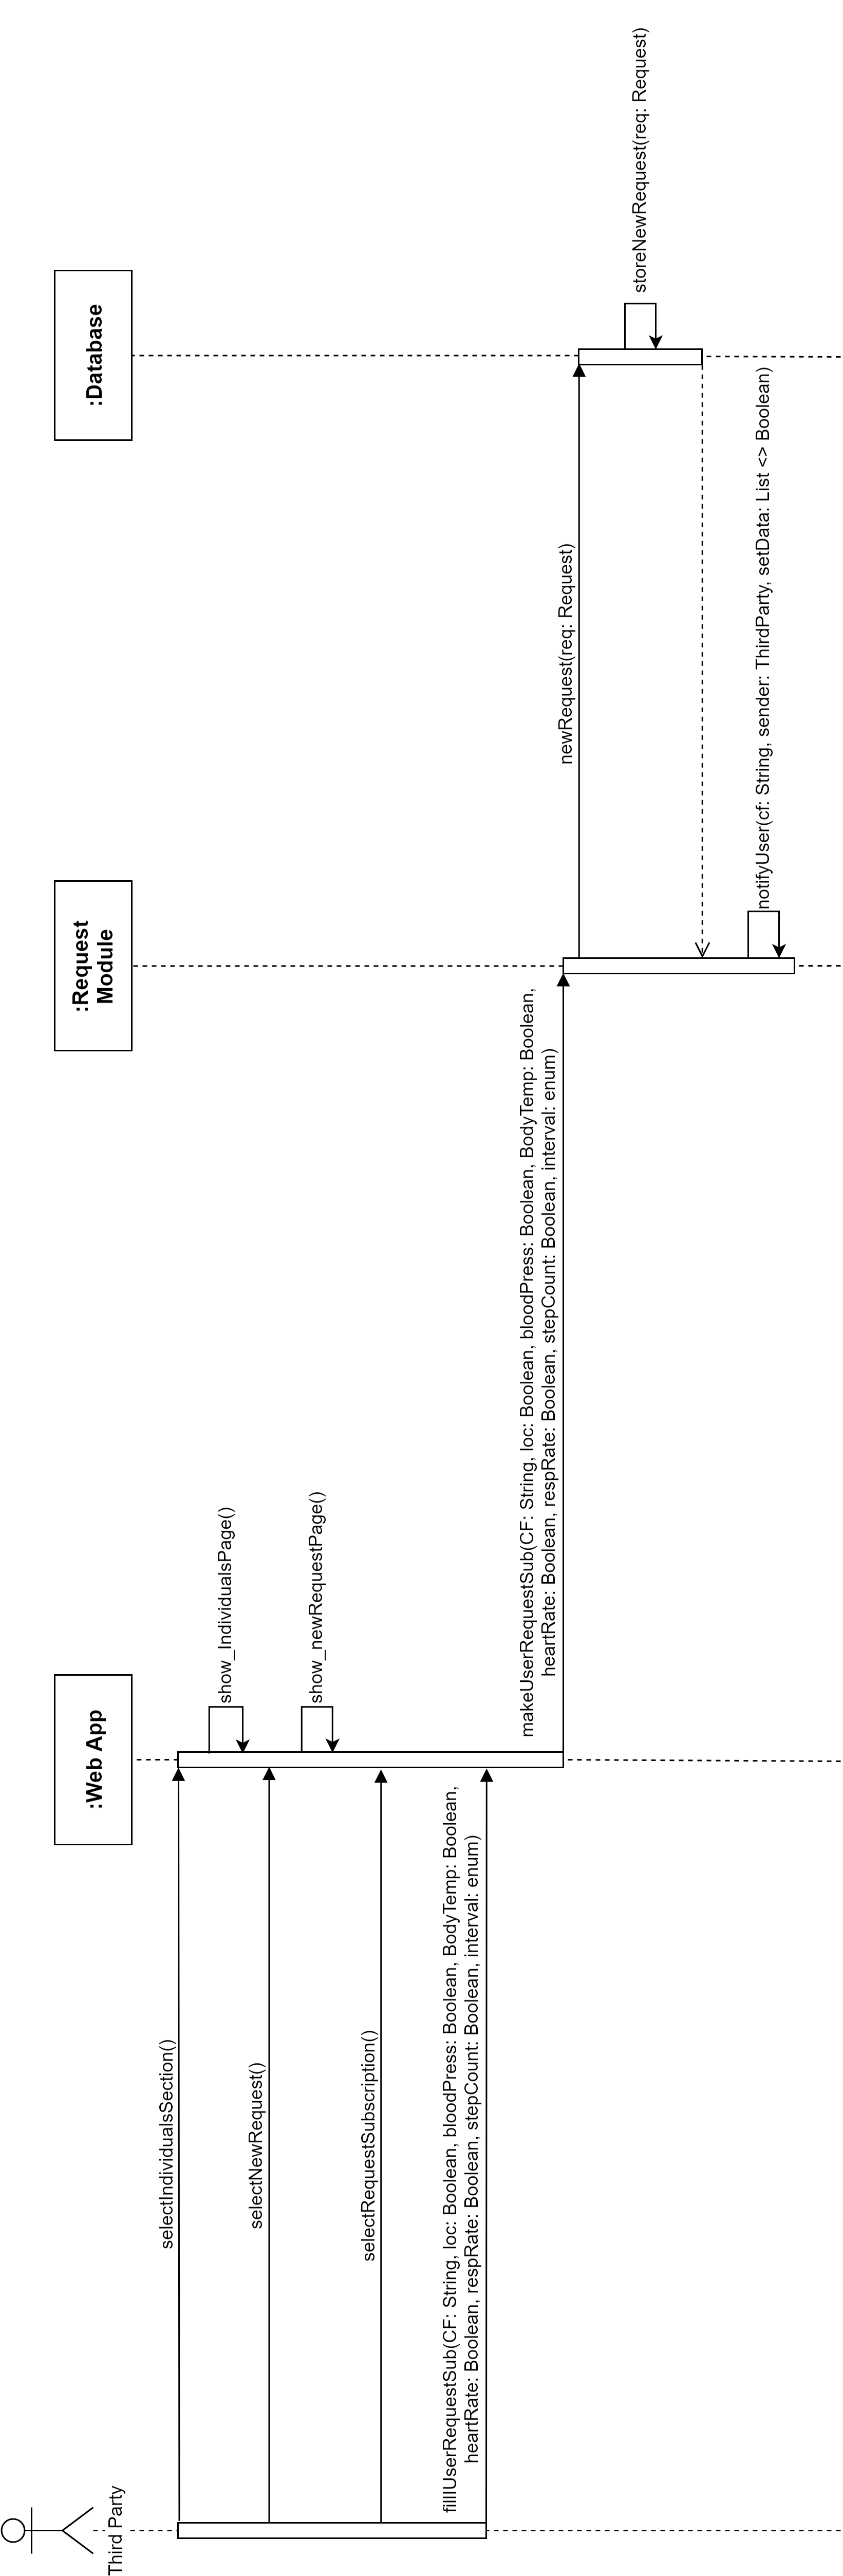
\includegraphics[scale=0.17]{DD/Pictures/userRequestV.png}
    \caption{User request by a Third Party}
\end{figure}

\begin{figure}[H]
    \centering
    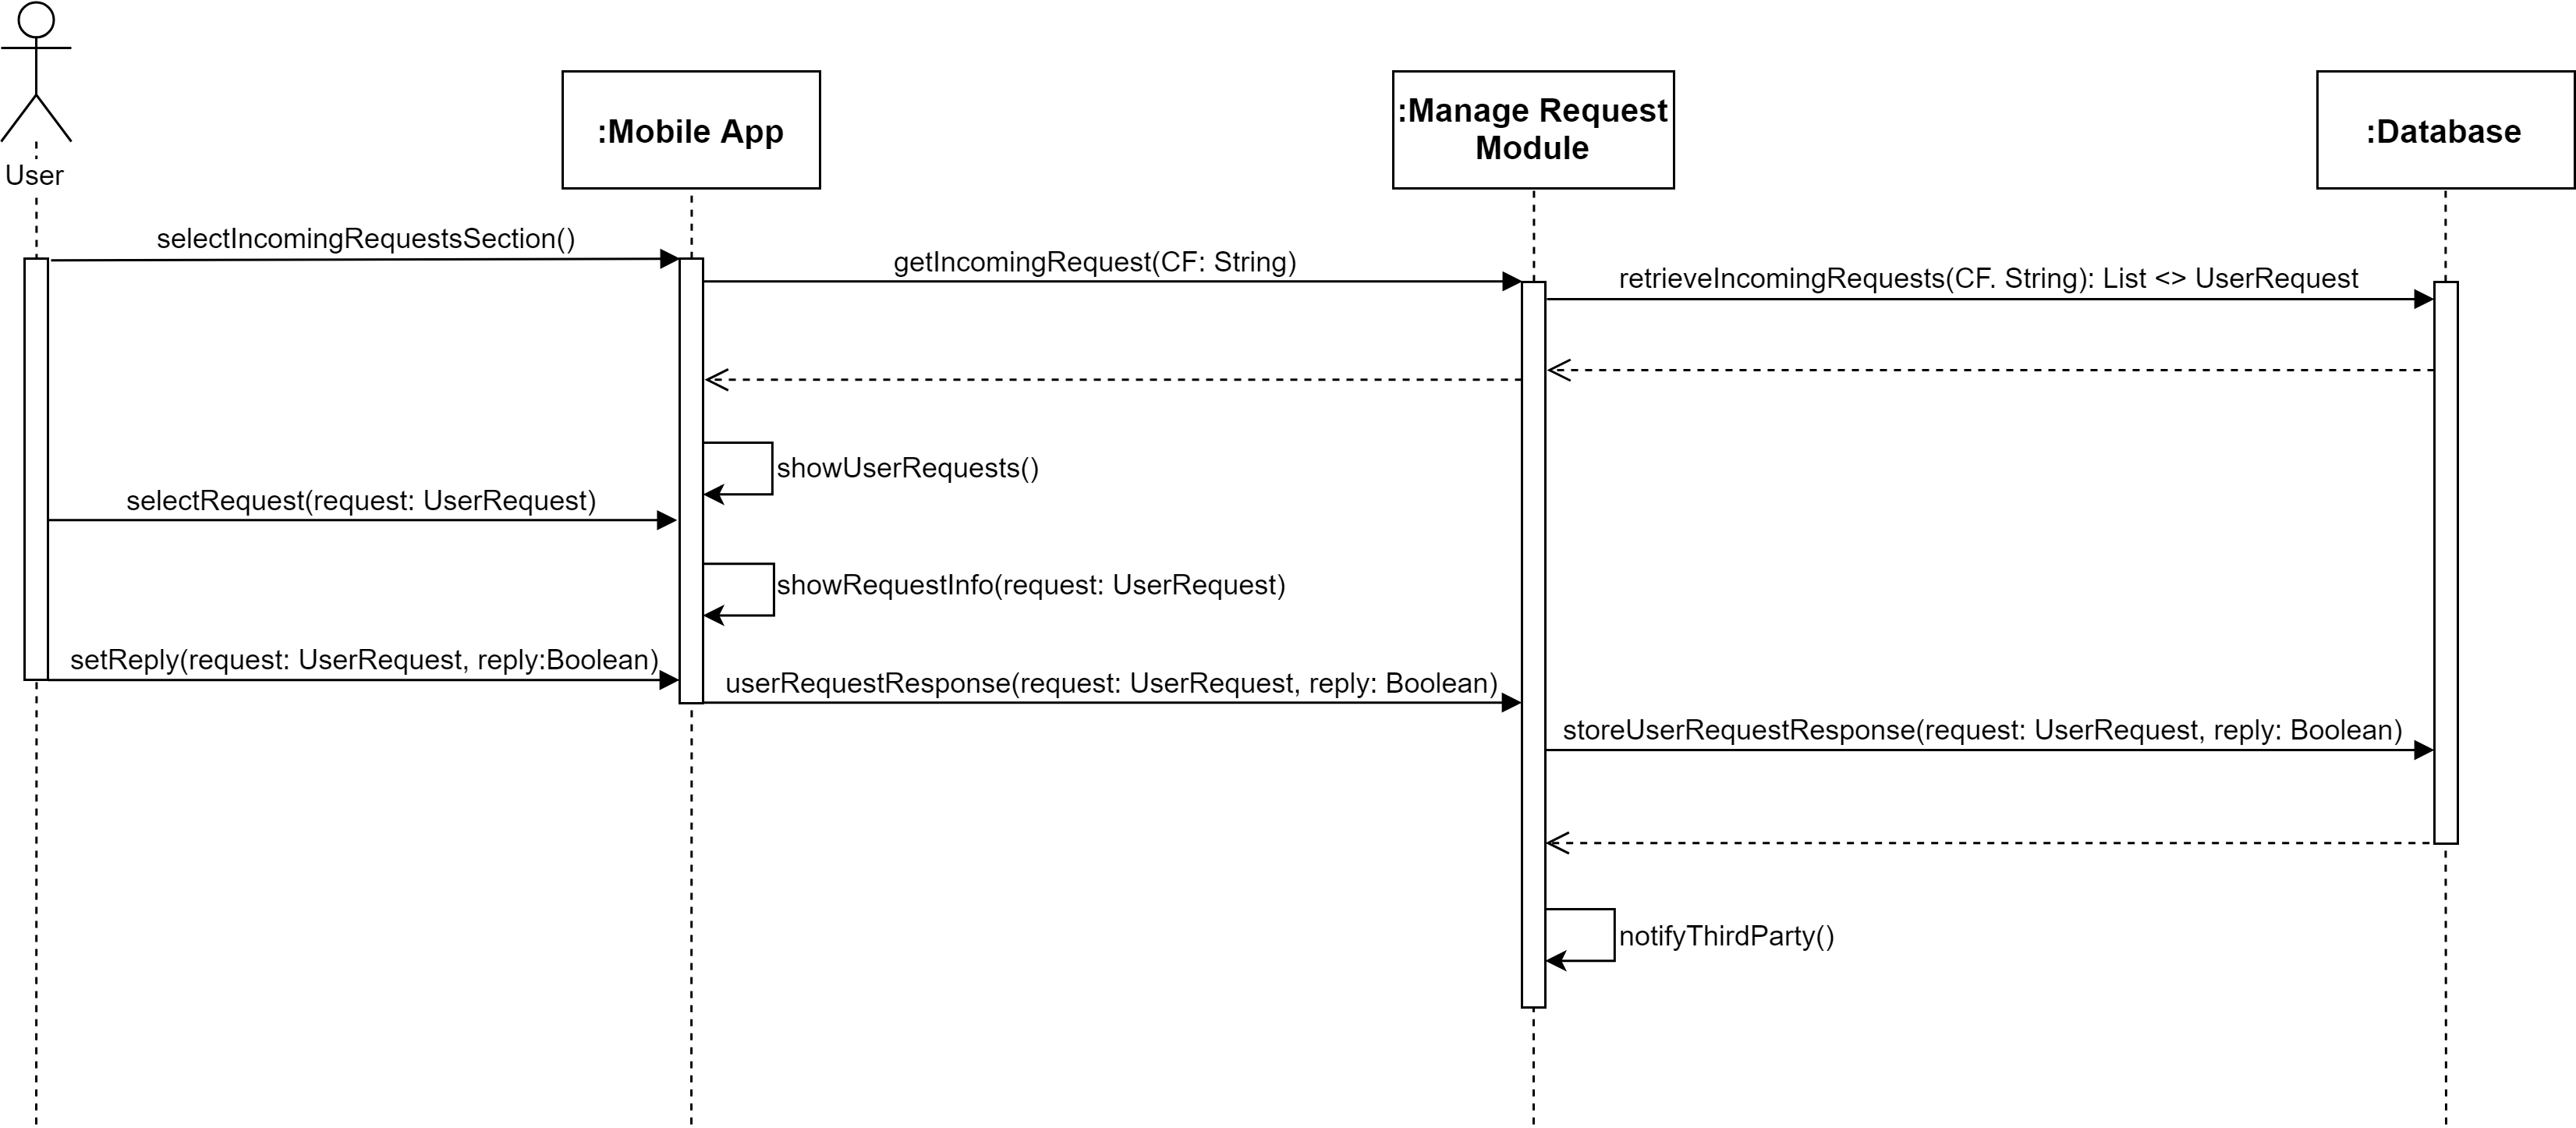
\includegraphics[scale=0.15]{DD/Pictures/acceptRequest.png}
    \caption{User acceptance of a request}
\end{figure}

\begin{figure}[H]
    \centering
    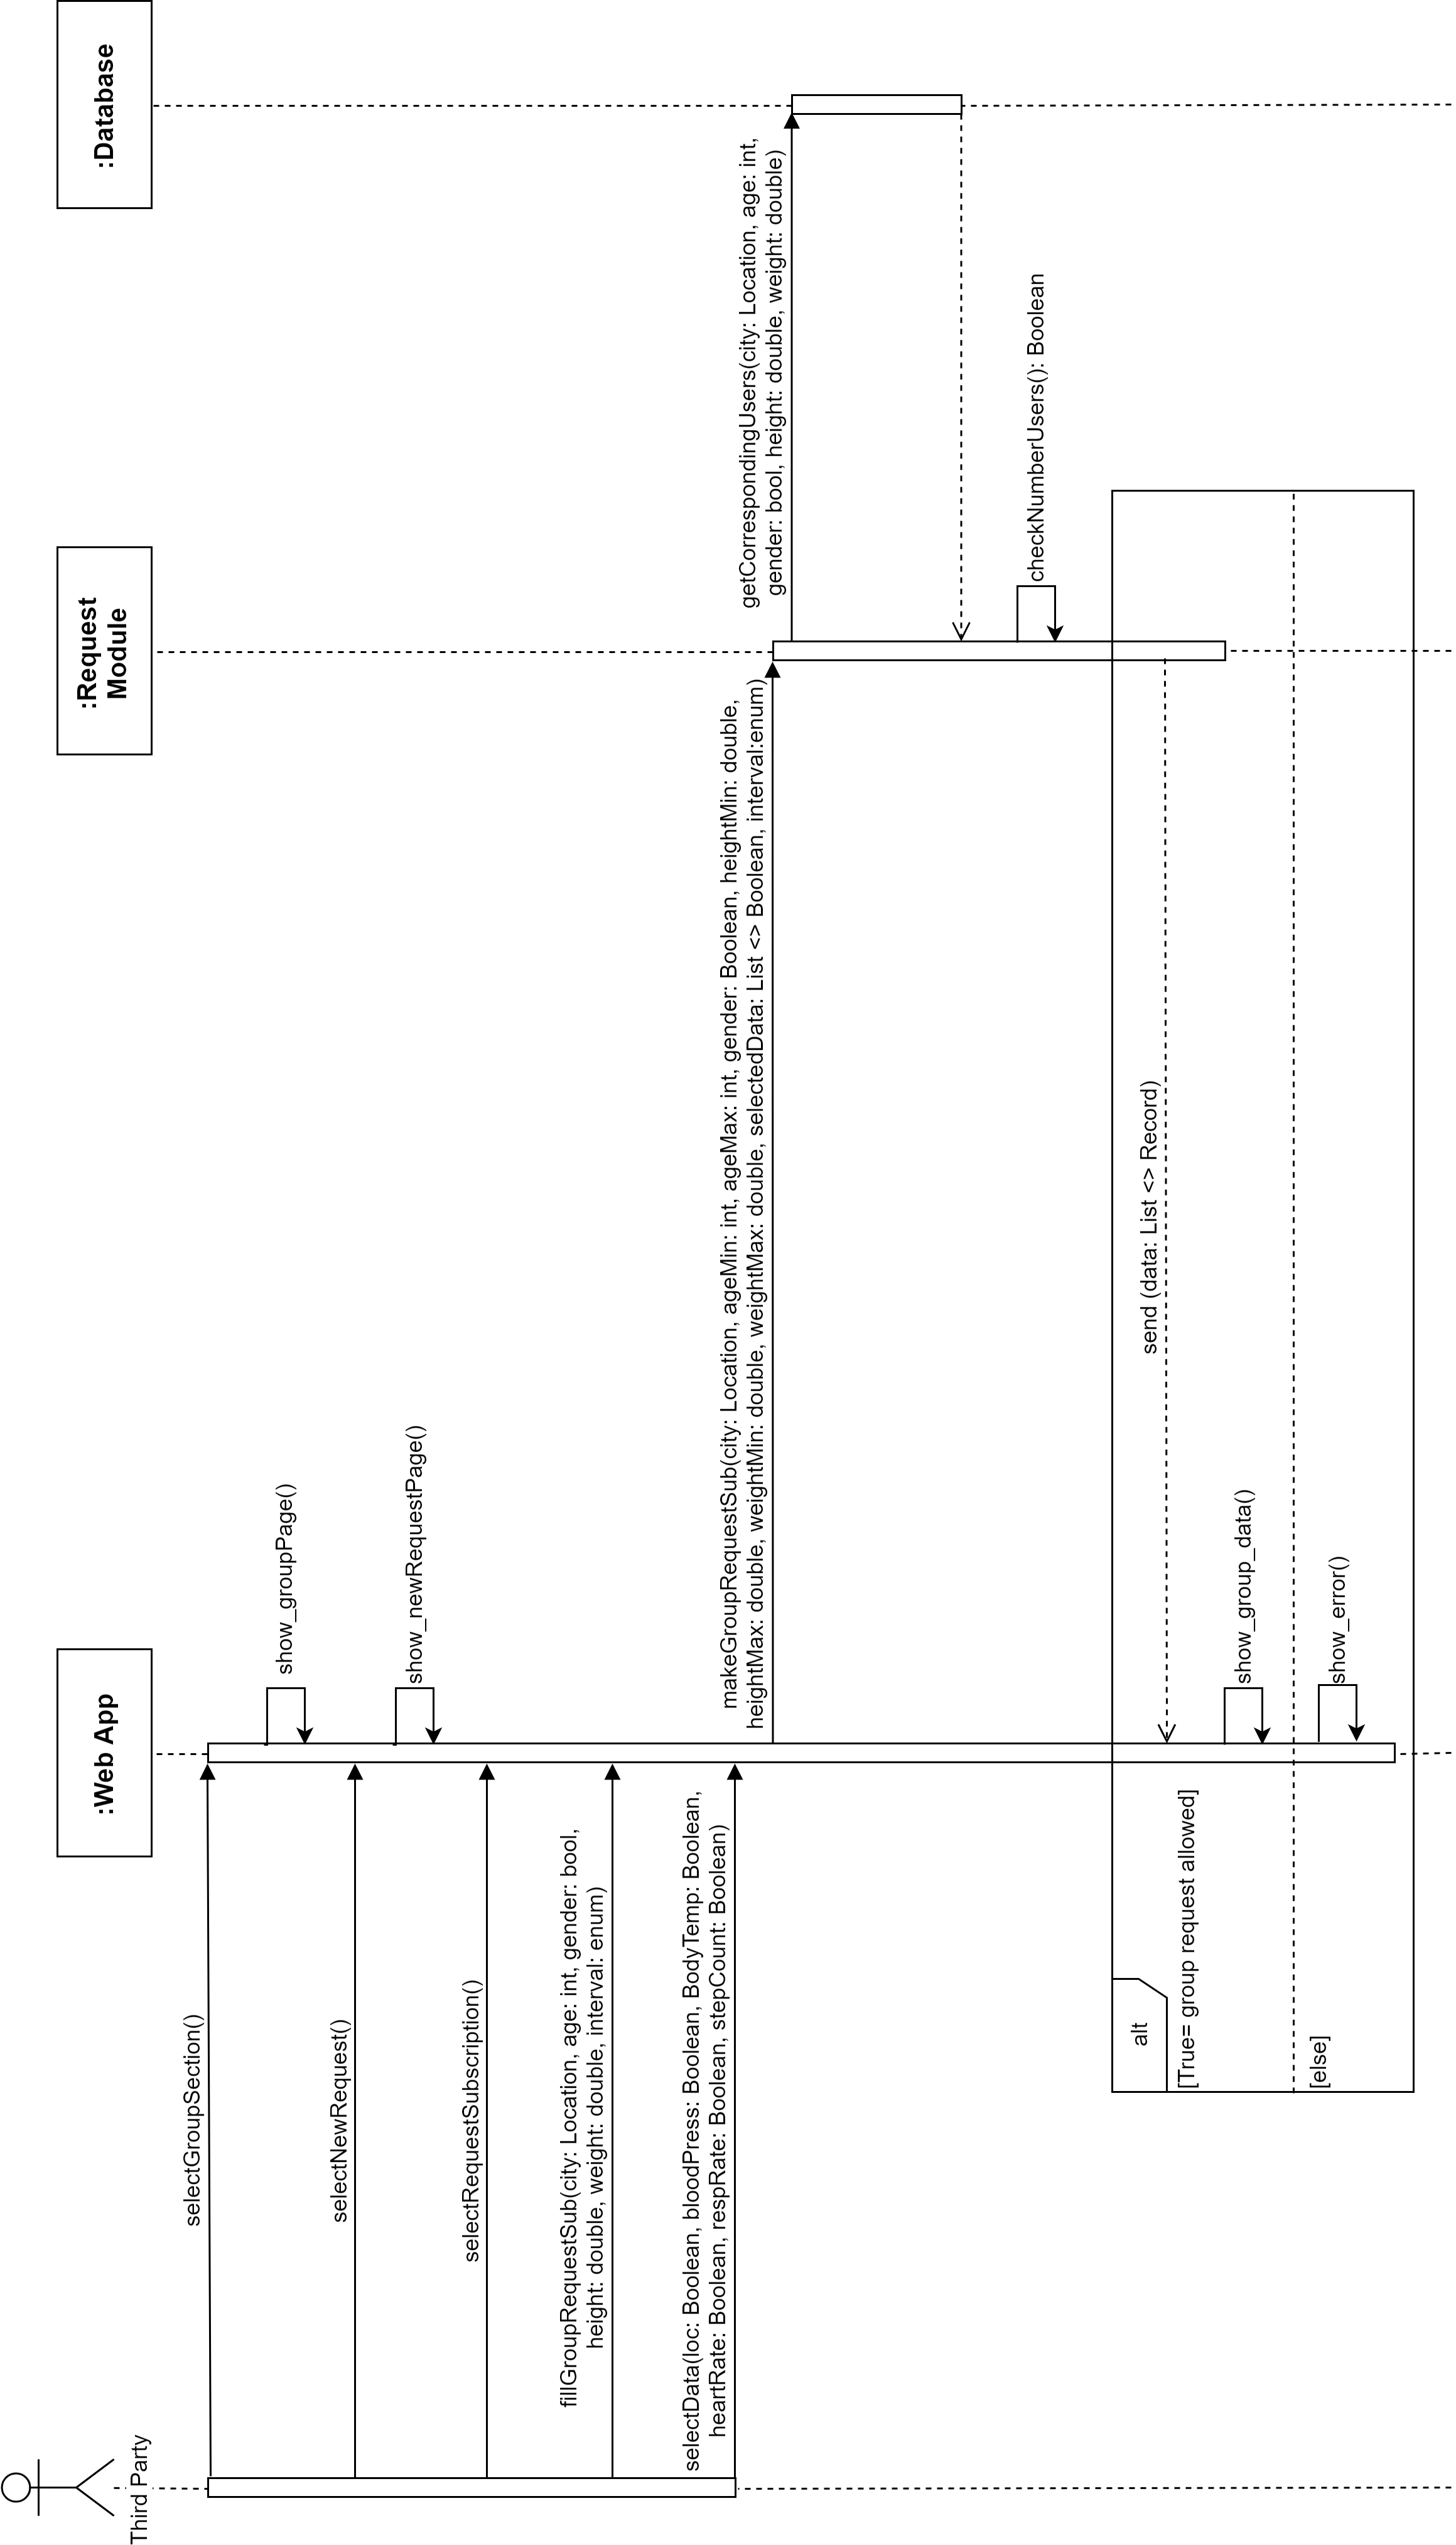
\includegraphics[scale=0.21]{DD/Pictures/groupRequestSeqDiagDDV.png}
    \caption{Group request by a Third Party}
\end{figure}

\begin{figure}[H]
    \centering
    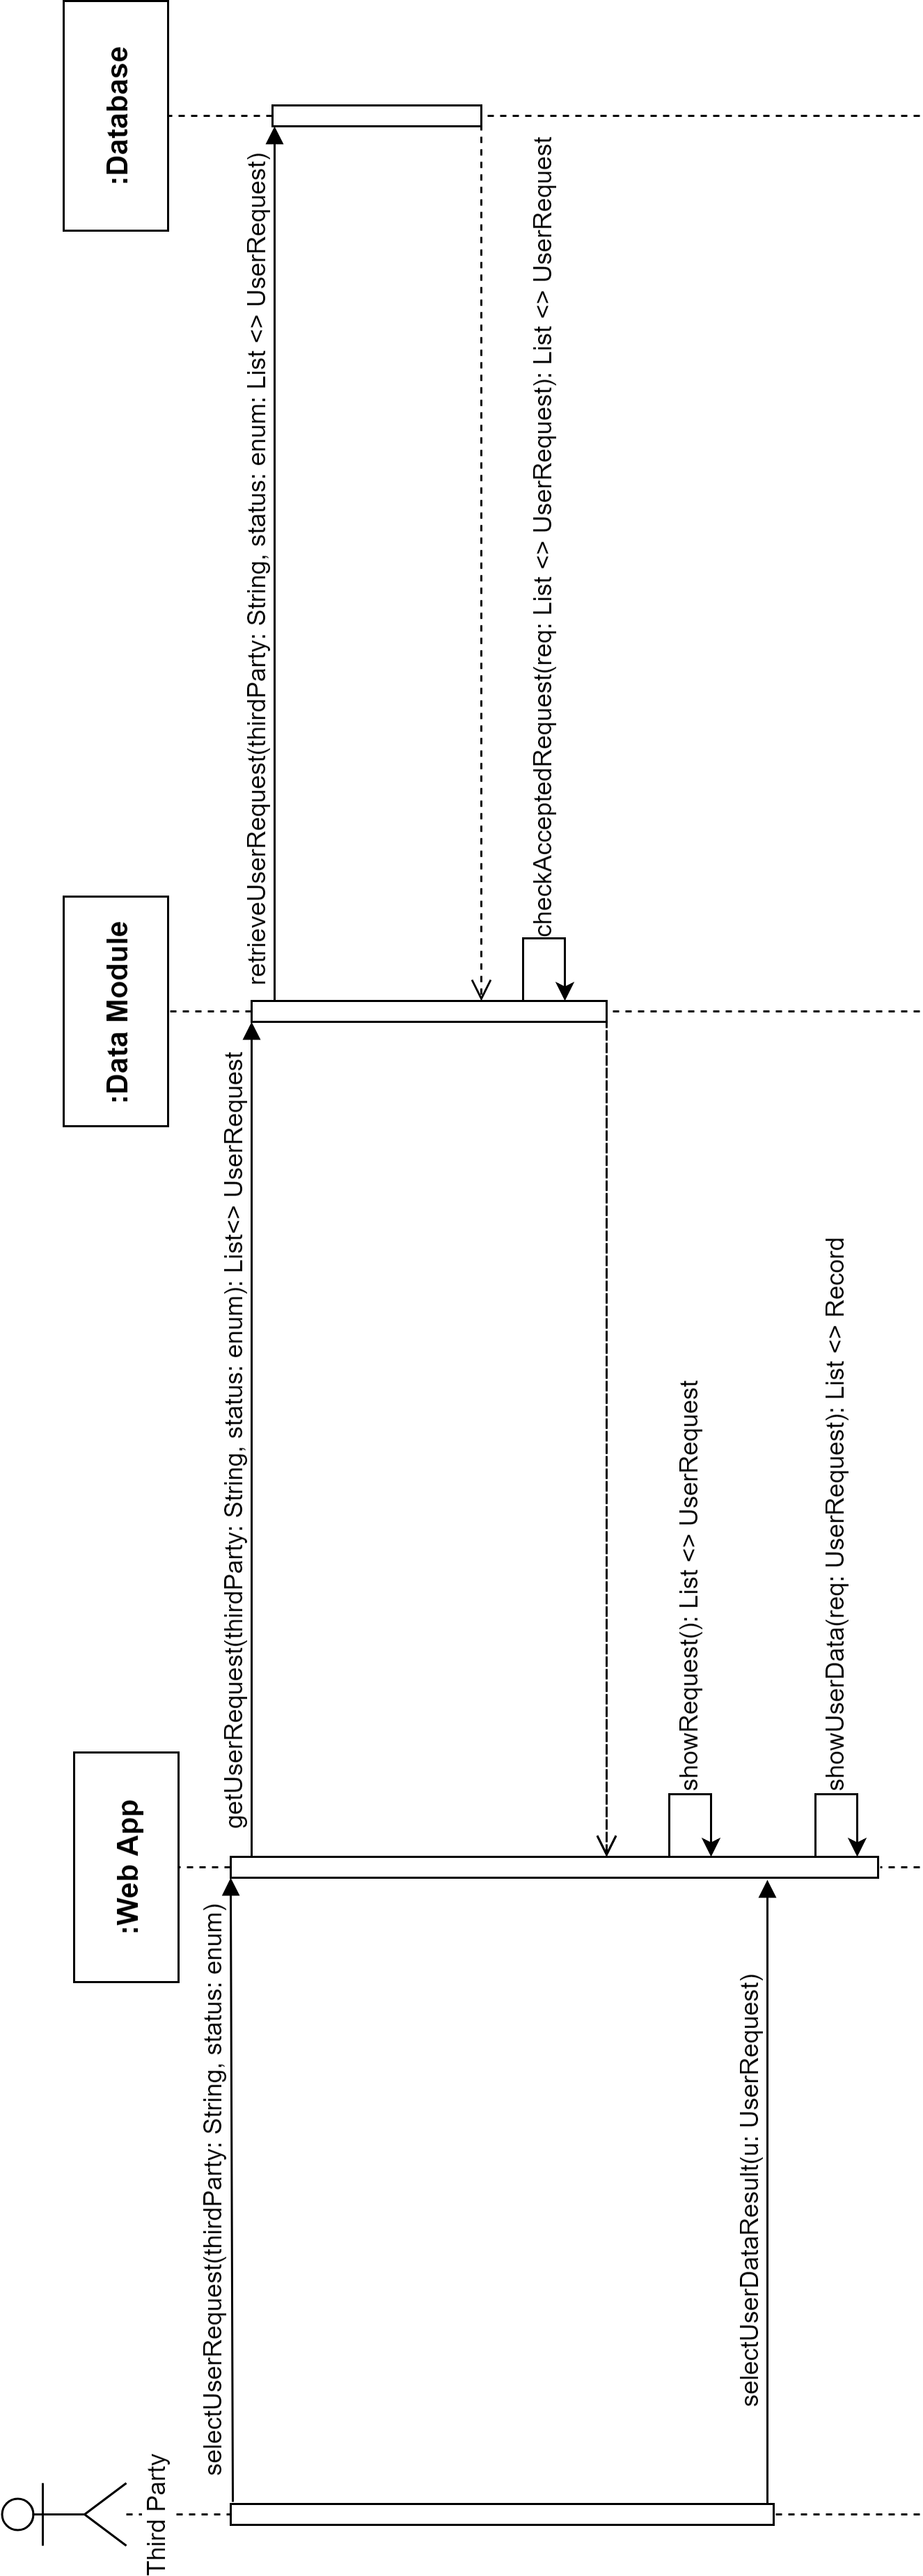
\includegraphics[scale=0.22]{DD/Pictures/showDataResultV.png}
    \caption{Visualization of data of a User that has already accepted the request}
\end{figure}

%emergency sequence diagram

\begin{figure}[H]
    \centering
    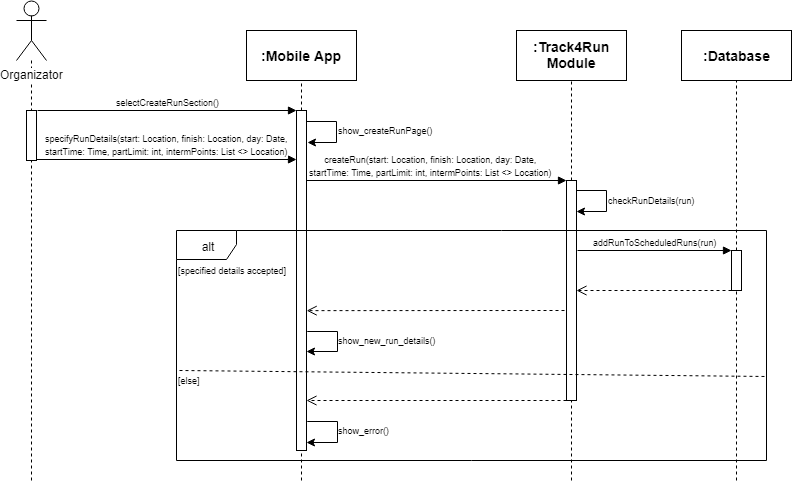
\includegraphics[scale=0.16]{DD/Pictures/createRunSeqDiagDD.png}
    \caption{Create a new run by an Organizer}
\end{figure}

\begin{figure}[H]
    \centering
    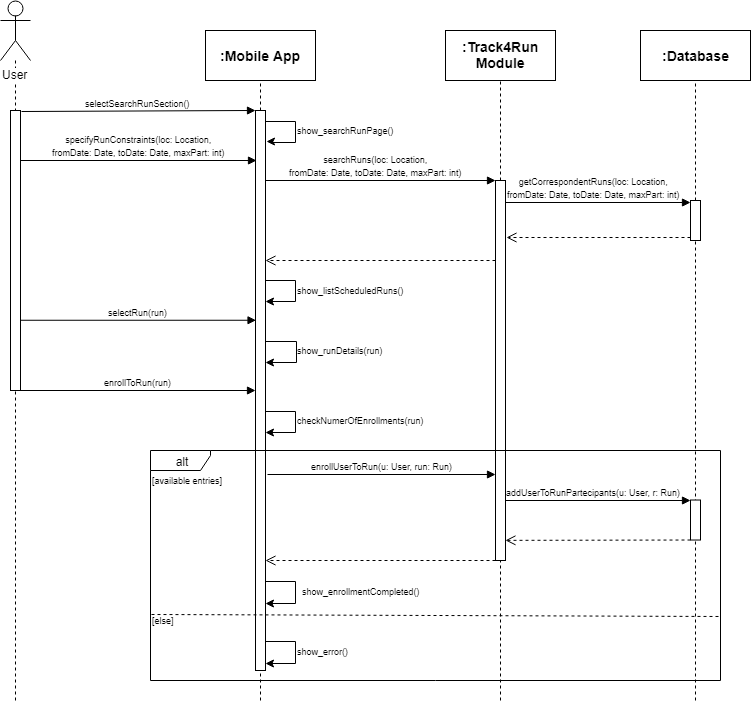
\includegraphics[scale=0.18]{DD/Pictures/enrollSeqDiagDD.png}
    \caption{Enrollment to a scheduled run by a User}
\end{figure}